\documentclass[10pt, compress]{beamer}

\usetheme{glasgow}

\usepackage{booktabs}
\usepackage[scale=2]{ccicons}
\usepackage{minted}
\usepackage{bookmark}
\usepgfplotslibrary{dateplot}

\usemintedstyle{trac}

% ($ (A)!r!(B) $) the location of images to be used
\graphicspath{{src/}}

%% Customisation
% \newcommand{\V}[1]{\v} % vectors \v{c}
% \renewcommand{\v}[1]{\mathbf{#1}} % vectors
\newcommand{\ti}[1]{\tilde{#1}} % spectral representation
\newcommand{\tnsr}[1]{\underline{\underline{#1}}}

% Symbols
\renewcommand{\O}{\omega}  % omega
\newcommand{\E}{\varepsilon}  % epsilon
\renewcommand{\u}{\mu}  % mu
\newcommand{\p}{\rho}  % rho
\newcommand{\x}{\times}  % times
\renewcommand{\inf}{\infty}  % infinity
\newcommand{\infint}{\int\limits_{-\inf}^\inf} % integral by R
\newcommand{\e}{\mathrm{e}} % Straight-up exponential
\renewcommand{\j}{{j}\mkern1mu} % Straight-up exponential
\newcommand{\iu}{\mathrm{i}\mkern1mu}

\newcommand\ddfrac[2]{\frac{\displaystyle #1}{\displaystyle #2}}

\title{High Frequency Communication Systems}
\subtitle{Lecture 4}
\date{Spring 2021}
\author{Hasan T Abbas \& Qammer H Abbasi}
% \institute{}

\begin{document}

\maketitle

%%%%%%%%%%%%%%%%%%%%%%%%%%%%%%%%%%%%%%%%%%
%%%%%%%%%%%%%%%%%%%%%%%%%%%%%%%%%%%%%%%%%%
%%%%%%%%%%%%%%%%%%%%%%%%%%%%%%%%%%%%%%%%%%
\begin{frame}[fragile]
  \frametitle{Lecture Outline}
\begin{outline}[itemize]
  \1 Transmission Lines Theory \& Analysis
  \1 Load Mismatching
  \1 The Magic of Quarter-wave Transformer
\end{outline}
\end{frame}
%%%%%%%%%%%%%%%%%%%%%%%%%%%%%%%%%%%%%%%%%%
%%%%%%%%%%%%%%%%%%%%%%%%%%%%%%%%%%%%%%%%%%
%%%%%%%%%%%%%%%%%%%%%%%%%%%%%%%%%%%%%%%%%%
\begin{frame}[fragile]
\frametitle{Transmission Line Theory}
\begin{outline}
  \1 A technique to bridge the gap between basic circuit analysis and electromagnetic fields theory
   \2 Lots of similarities and analogies
    \1 Commonly used to design microwave devices and circuits
    \1 We use transmission lines when the electrica length of the device is greater than $\lambda / 10$.
\end{outline}
\end{frame}

\begin{frame}
  \frametitle{TL \& EM Field Theory - Duality}
  \begin{columns}[T] % align columns
  \begin{column}{.3\textwidth}
\begin{outline}
  \1 In wave scattering problems, we place the co-ordinate system at the boundary
  \1 In transmission lines, we use the two different lines as the boundary
  \1 For open problems, the load is considered to be at infinity.
  \end{outline}
   \end{column}
 \begin{column}[T]{.7\textwidth}
    \begin{figure}
      \centering
          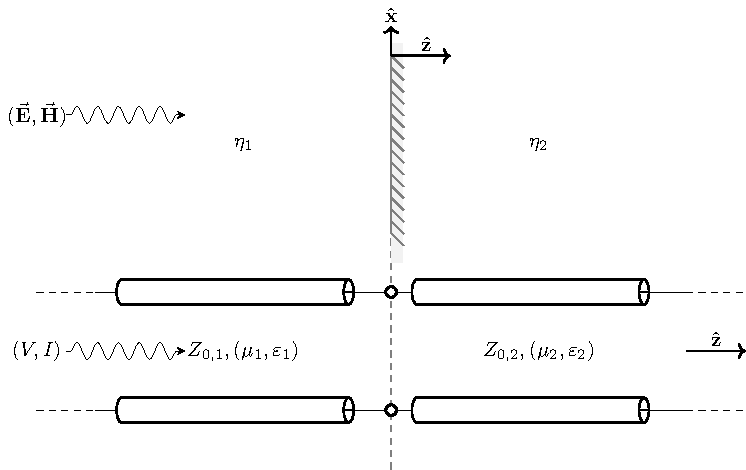
\includegraphics[width=.9\textwidth]{circuit.pdf}
      \caption{The analogy between wave problems and transmission lines.}
    \end{figure}
      \end{column}%
\end{columns}
  \end{frame}


\begin{frame}
  \frametitle{TL \& EM Field Theory Duality}
  \begin{table}
    \begin{tabular}{ll}
    \toprule
    TL Theory & EM Field Theory \\
    \midrule
    $V_{1} = V_{0} \e^{-\j \gamma_{1} z} \left(1+\Gamma_{L} \e^{\j 2 \gamma_{1} z}\right)$ & $E_{x,1}=E_{0} \e^{-\j k_{1} z} \left( 1 + \Gamma \e^{\j 2 k_{1} z} \right)$ \\
    $I_{1} = \frac{V_{0}}{Z_{0,1}} \e^{-\j \gamma_{1} z} \left(1+\Gamma_{L} \e^{\j 2 \gamma_{1} z}\right)$ & $H_{x,1} = \frac{E_{0}}{\eta_0} \e^{-\j k_{1} z} \left( 1 + \Gamma \e^{\j 2 k_{1} z} \right)$ \\
   $ \Gamma_{L} = \frac{Z_L - Z_{0,1}}{Z_L + Z_{0,1}} = \frac{Z_{0,2} - Z_{0,1}}{Z_{0,2} + Z_{0,1}}$ & $\Gamma = \frac{\eta_2 - \eta_1}{\eta_2 + \eta_1}$ \\
   $V_2 = T V_0 \e^{-\j \gamma_{2} z}$ & $E_{x,2} = T E_0 \e^{-\j k_{2} z}$ \\
   $I_2 = T \frac{V_0}{Z_{0,2}} \e^{-\j \gamma_{2} z}$ & $H_{x,2} = T \frac{E_0}{\eta_2} \e^{-\j k_{2} z}$ \\
   $T = \frac{2 Z_{0,2}}{{Z_{0,2}} + {Z_{0,1}}}$ & $T = \frac{2 \eta_2}{\eta_2 + \eta_1}$ \\
   \bottomrule
  \end{tabular}
\end{table}
\end{frame}


\begin{frame}
  \frametitle{TL Theory and Circuit Elements}
\begin{outline}
  \1 For a transmission line, we use a distributed circuit approach
  \2 Energy stored in the magnetic field $\rightarrow L$
  \2 Energy stored in the electric field $\rightarrow C$
  \2 Conductive losses $\rightarrow R$
  \2 Dielectric losses $\rightarrow G$
  \1 All the circuit elements are expressed per unit length
  \1 We can express the voltage and current at any given point $z$ and time $t$.
\end{outline}
\end{frame}

\begin{frame}
  \frametitle{The Transmission Line Equation}

\begin{figure}
  \centering
  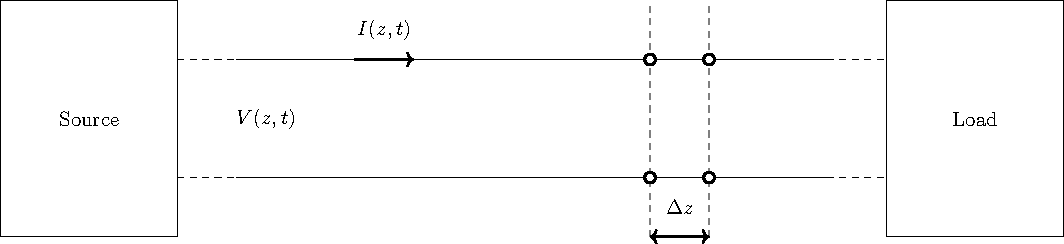
\includegraphics[width=.85\textwidth]{tlines.pdf}
  \end{figure}
  \begin{figure}
    \centering
    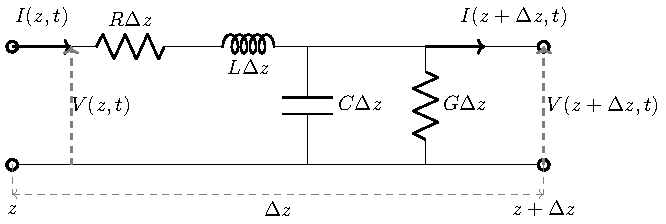
\includegraphics[width=.85\textwidth]{circuit2.pdf}
      \end{figure}
\end{frame}

\begin{frame}
  \frametitle{Solution to the Transmission Line Equation - The Telegraphers Equation}
\begin{outline}
  \1 Solving the electric circuit leads to a second order differential equation
  \1 Analogous to the wave equation
  \2 Hence the analogies between voltage $V$ and electric field $\va{E}$
\end{outline}
\begin{align*}
  \left\{ \pdv[2]{z} - \left[ (R + \j \O L)( G + \j \O C)  \right] \right\} V (z,t) = 0
\end{align*}
The solution is of the type:
\begin{align*}
  V(z) &= V_{+} \e^{-\gamma z} + V_{-} \e^{+\gamma z}
\end{align*}
where the propagation constant $\gamma = \sqrt{(R + \j \O L)( G + \j \O C)}$. For a lossless case $R = G = 0$. 
\end{frame}

\begin{frame}
  \frametitle{Equivalent Circuits - Terminated Load}
\begin{outline}
  \1 For a transmission line terminated with a load $Z_L$
  \2 We get reflections in the line (superposition incoming and reflected wave make up the total voltage)
  \1 The input impedance depends on the $Z_L$ as well as the length $l$ of the transmission line
  \1 For Transmission line analysis, we shift the origin to the load.
\end{outline}

  \begin{figure}[H!]
    \centering
    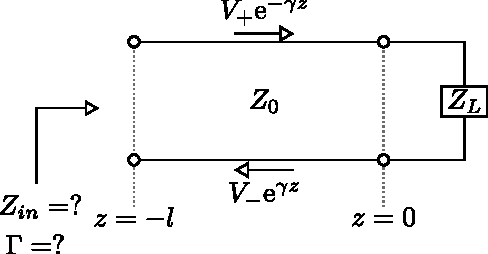
\includegraphics[width=.8\textwidth]{tline_terminated.pdf}
  \end{figure}

\end{frame}

\begin{frame}
  \frametitle{TL with Terminated Load}
  The \textit{voltage reflection coefficient} $\Gamma$ can for the line is
  \begin{align*}
    \Gamma &= \frac{V_{ref}}{V_{inc}} = \frac{V_{-} \e^{\gamma z}}{V_{+} \e^{-\gamma z}} \\
    &= \frac{V_{-,z = 0}}{V_{+,z = 0}} \e^{2 \gamma z} = \Gamma_L \e^{2 \gamma z}
  \end{align*}
  We can express the voltage at any point on the line as:
\begin{align*}
  V(z) &= V_{+} \left( \e^{- \gamma z} + \Gamma_L \e^{ \gamma z} \right)
\end{align*}
After finding a similar expression for the current, we can write the impedance as:
\begin{align*}
  Z(z) &= Z_0 \frac{\e^{-\gamma z} + \Gamma_L \e^{-\gamma z}}{\e^{-\gamma z} - \Gamma_L \e^{-\gamma z}}
\end{align*}
At $z = 0$, $Z(0) = Z_L$, and we get:
\begin{align*}
  Z_L = Z_0 \frac{1 + \Gamma_L}{1 - \Gamma_L} \implies \Gamma_L &= \frac{Z_L - Z_0}{Z_L + Z_0}
\end{align*}
\end{frame}

\begin{frame}
  \frametitle{TL Impedance}
At $z = -l$, the input impedance $Z(-l) - Z_{in}$ is given by:
\begin{align*}
  Z(-l) &= Z_0 \frac{\e^{\gamma l} + \e^{-\gamma l}\Gamma_L}{\e^{\gamma l} - \e^{\gamma l}\Gamma_L} \\
  &= Z_0 \frac{\left(Z_L + Z_0\right)\e^{\gamma l} + \left(Z_L - Z_0\right) \e^{-\gamma l}}{\left(Z_L + Z_0\right)\e^{\gamma l} - \left(Z_L - Z_0\right) \e^{-\gamma l}} \\
  &= Z_0 \frac{Z_L + Z_0 \tanh{\gamma l}}{Z_0 + Z_L \tanh{\gamma l}}
\end{align*}

For lossless TLs $\gamma = \j \beta$, therefore,
\begin{align*}
Z(-l) &= Z_0 \frac{Z_L + \j Z_0 \tan{\beta l}}{Z_0 + \j Z_L \tan{\beta l}}  
\end{align*}
\end{frame}

\begin{frame}
  \frametitle{Special Cases of Load Impedance - Short Circuit}
  \begin{columns}[T] % align columns
    \begin{column}{.4\textwidth}
      For $Z_L = 0$,
      \begin{align*}
        Z_{in} &= Z_0 \j \tan (\beta l) \\
        \Gamma_{in} &= -1 
      \end{align*}
      \begin{figure}[h!]
        \centering
        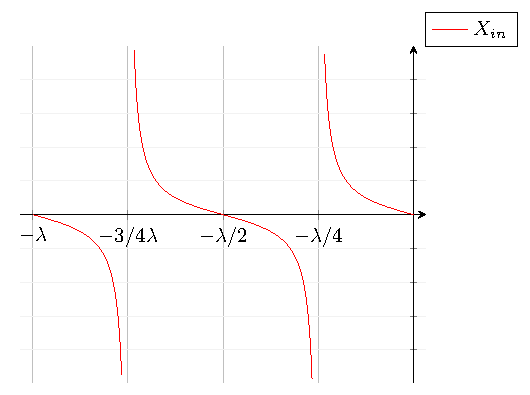
\includegraphics[width=.95\textwidth]{short_impedance.pdf}
      \end{figure}
     \end{column}
   \begin{column}[T]{.6\textwidth}
    \begin{figure}[T!]
      \centering
      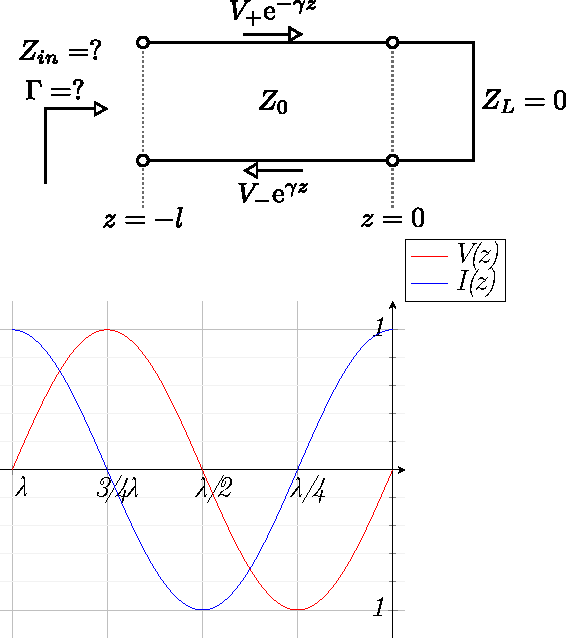
\includegraphics[width=.9\textwidth]{tline_short.pdf}
      \end{figure}
        \end{column}%
  \end{columns}
\end{frame}


\begin{frame}
  \frametitle{Special Cases of Load Impedance - Open Circuit}
  \begin{columns}[T] % align columns
    \begin{column}{.4\textwidth}
      For $Z_L = \infty$,
      \begin{align*}
        Z_{in} &=  - Z_0 \j \cot (\beta l) \\
        \Gamma_{in} &= 1 
      \end{align*}
      \begin{figure}[h!]
        \centering
        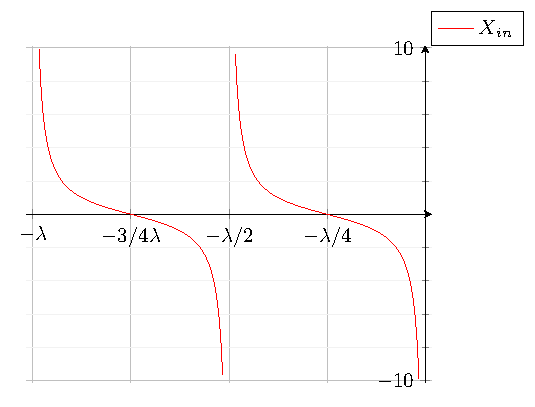
\includegraphics[width=.95\textwidth]{open_impedance.pdf}
      \end{figure}
     \end{column}
   \begin{column}[T]{.6\textwidth}
    \begin{figure}[T!]
      \centering
      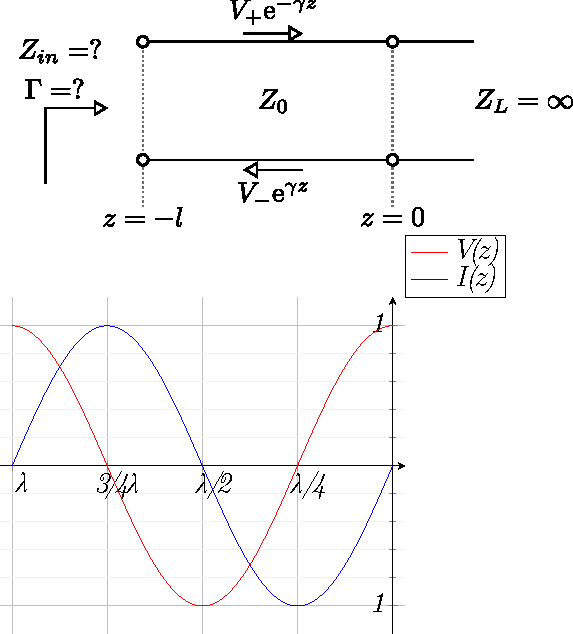
\includegraphics[width=.9\textwidth]{tline_open.pdf}
      \end{figure}
        \end{column}%
  \end{columns}
\end{frame}


\begin{frame}
  \frametitle{Special Cases of Load Impedance - Matched Load}
  \begin{columns}[T] % align columns
    \begin{column}{.3\textwidth}
      For $Z_L = Z_0$,
      \begin{align*}
        Z_{in} &=   Z_0  \\
        \Gamma_{in} &= 0 
      \end{align*}
     \end{column}
   \begin{column}[T]{.7\textwidth}
    \begin{figure}[T!]
      \centering
      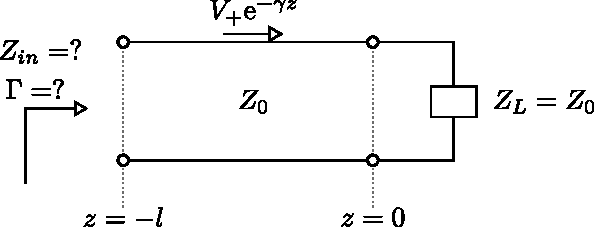
\includegraphics[width=.9\textwidth]{tline_matched.pdf}
      \end{figure}
        \end{column}%
  \end{columns}
  \begin{outline}
    \1 Ideally we desire this condition for maximum power transfer.
    \1 No reflections take place in this case
  \end{outline}
\end{frame}

\begin{frame}
  \frametitle{Special Cases of Load Impedance - The Quarter-wave Transformer}
    \begin{outline}
    \1 We see that for terminated loads with special lengths that are multiples of quarter wavelengths ($\lambda/4 + n \lambda/2$) for $n = 1,2,3, \cdots$
    \1 The load impedance is inverted
      \2 Open-circuit load becomes short-circuit and vice versa
    \1 For such a line, the input impedance is $Z_{in} = \frac{Z_0^2}{Z_L}$
  \end{outline}
  \begin{figure}[h!]
    \centering
    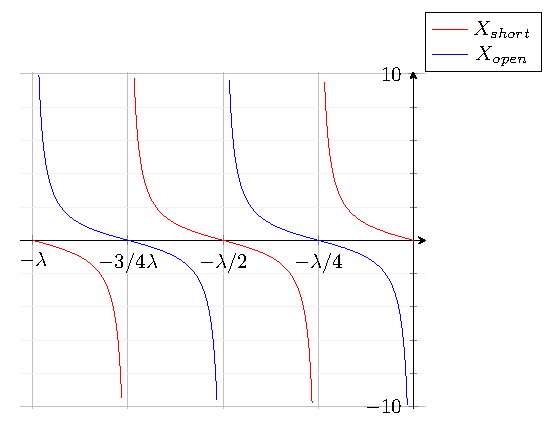
\includegraphics[width=.6\textwidth]{invert_impedance.pdf}         
  \end{figure}
\end{frame}

\begin{frame}
  \frametitle{The Voltage Standing Wave Ratio}
\begin{outline}
  \1 We want maximum power transferred to the load from the transmission line.
  \2 For that to happen, we require the impedance matching of the transmission line.
  \1 The reflections in the TL are undesirable and lead to a standing wave generation ($V = V_{+} + V_{-}$).
  \1 The voltage standing wave ratio (VSWR) measures the quality of impedance matching in TL.
\end{outline}
\end{frame}

\begin{frame}
  \frametitle{The VSWR}

  Recall, 
  \begin{align*}
    V(z) &= V_{+} \left( \e^{- \gamma z} + \Gamma_L \e^{ \gamma z} \right)
  \end{align*}
  The values of the voltage reflection coefficient range from $-1 \le |\Gamma_L| \le 1$.

  The VSWR is the ratio of the maximum and minimum absolute values of the voltage
  \begin{align*}
    VSWR &= \frac{|V_{max}|}{|V_{min}|}
  \end{align*}
  In other words,
  \begin{align*}
    |V_{max}| &= V_0 \left(1 + |\Gamma_L|\right) \\
    |V_{min}| &= V_0 \left(1 - |\Gamma_L|\right) \\  
    VSWR &= \frac{1 + |\Gamma_L|}{1 - \Gamma_L}
  \end{align*}
\end{frame}

\begin{frame}
  \frametitle{Terminated Load - Example}
\begin{figure}[t!]
  \centering
  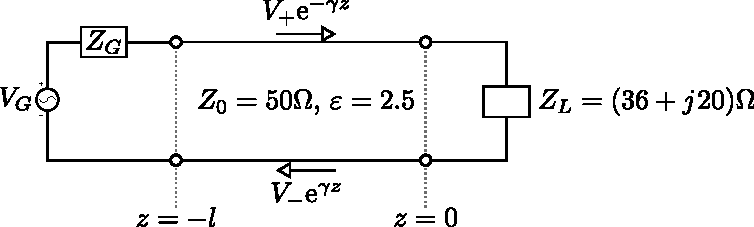
\includegraphics[width=.9\textwidth]{tline_terminated_example.pdf}
\end{figure}
  For the TL above with a length $l$ of $\SI{6.33}{\m}$, find the average power delivered to the load as well as the line. The source voltage is $V_G = \SI{100}{\volt}$ operating at a frequency of 200 MHz. The source impedance $Z_G$ is also $\SI{50}{\ohm}$. First, check whether the circuit is actually a transmission line. Also find the input impedance $Z_{in} = Z(-l)$ of the line.
\end{frame}

\begin{frame}
  \frametitle{Example - Solution}
First we check the electrical length of the transmission line.
  \begin{align*}
    \beta &= k = \frac{2 \pi}{\lambda} = \frac{\O}{v} \\
    & \implies \lambda = \frac{v}{f} = \frac{c}{\sqrt{\E_r} f} = \frac{\num{3e8}}{\sqrt{2.5} \times \num{20e6}} \\
    \lambda &= \SI{10.55}{\m} \implies l = \frac{6.33}{10.55} = 0.6 \lambda
  \end{align*}
As $l > 0.1 \lambda$, the given circuit can be treated as a transmission line.
\end{frame}


\begin{frame}
  \frametitle{Example Solution - The input impedance}

  As $Z_0$ is real-valued, we treat the TL as lossless.
  \begin{align*}
    Z_{in} = Z(-l) &= Z_0 \frac{Z_L + \j Z_0 \tan{\beta l}}{Z_0 + \j Z_L \tan{\beta l}}  \\
    &= 50 \times \frac{(36 + \j 20) + \j 50 \tan{(2 \pi \times 0.6)}}{50 +  \j (36 + \j 20) \tan{(2 \pi \times 0.6)}} \\
    Z_{in}&= \SI{86.15 - j10.93}{\ohm}
  \end{align*}

  
\end{frame}
\begin{frame}
  \frametitle{Example Solution - Power calculation}

  The equivalent circuit now looks like:
  \begin{figure}[H!]
    \centering
    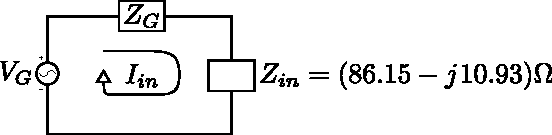
\includegraphics[width=.6\textwidth]{tline_terminated_example_power.pdf}
  \end{figure}
  The current in the circuit is:
  \begin{align*}
    I_{in} &= \frac{V_G}{Z_G + Z_{in}} \\
    &= \frac{100}{50 + 86.15 - \j 10.93} = \SI{0.73 + j 0.06}{\ampere}
  \end{align*}
  The average input power is:
  \begin{align*}
    P_{in} &= 1/2 \Re{V_{in} I_{in}^*} = 1/2 \Re{Z_{in} I_{in} I_{in}^*} = \SI{23.09}{\watt} 
  \end{align*}

\end{frame}
\begin{frame}
  \frametitle{Example Solution - Load Power}
We first calculate the current $I(z)$ in the transmission line.
\begin{align*}
  I(z) &= \frac{V_{+}}{Z_0} \left( e^{-\j \beta z} - \Gamma e^{\j \beta z}\right) 
\end{align*}
At $z = -l$, $I(-l) = I_{in}$ and treating $\frac{V_{+}}{Z_0} = I_{+}$
\begin{align*}
  I(-l) = I_{in} &= I_{+} \left( e^{+\j \beta l} - \Gamma_{in} e^{-\j \beta l}\right) \\
  I_{+} &= I_{in}/\left( e^{+\j \beta l} - \Gamma_{in} e^{-\j \beta l}\right)  = \SI{-0.47 + j 0.89}{\ampere}
\end{align*}
The current at the load is:
\begin{align*}
  I_L &= I_{+}(1 - \Gamma_L)
\end{align*}
The power at the load is hence:
\begin{align*}
  P_{load} &= 1/2 \Re\{I_{L} I_{L }^*Z_L\} \\
    &= \SI{23.09}{\watt}
\end{align*}
\end{frame}

% \section{The Smith Chart}
% \begin{frame}
%   \frametitle{The Smith Chart}
% \begin{figure}[htbp]
%   \centering
%   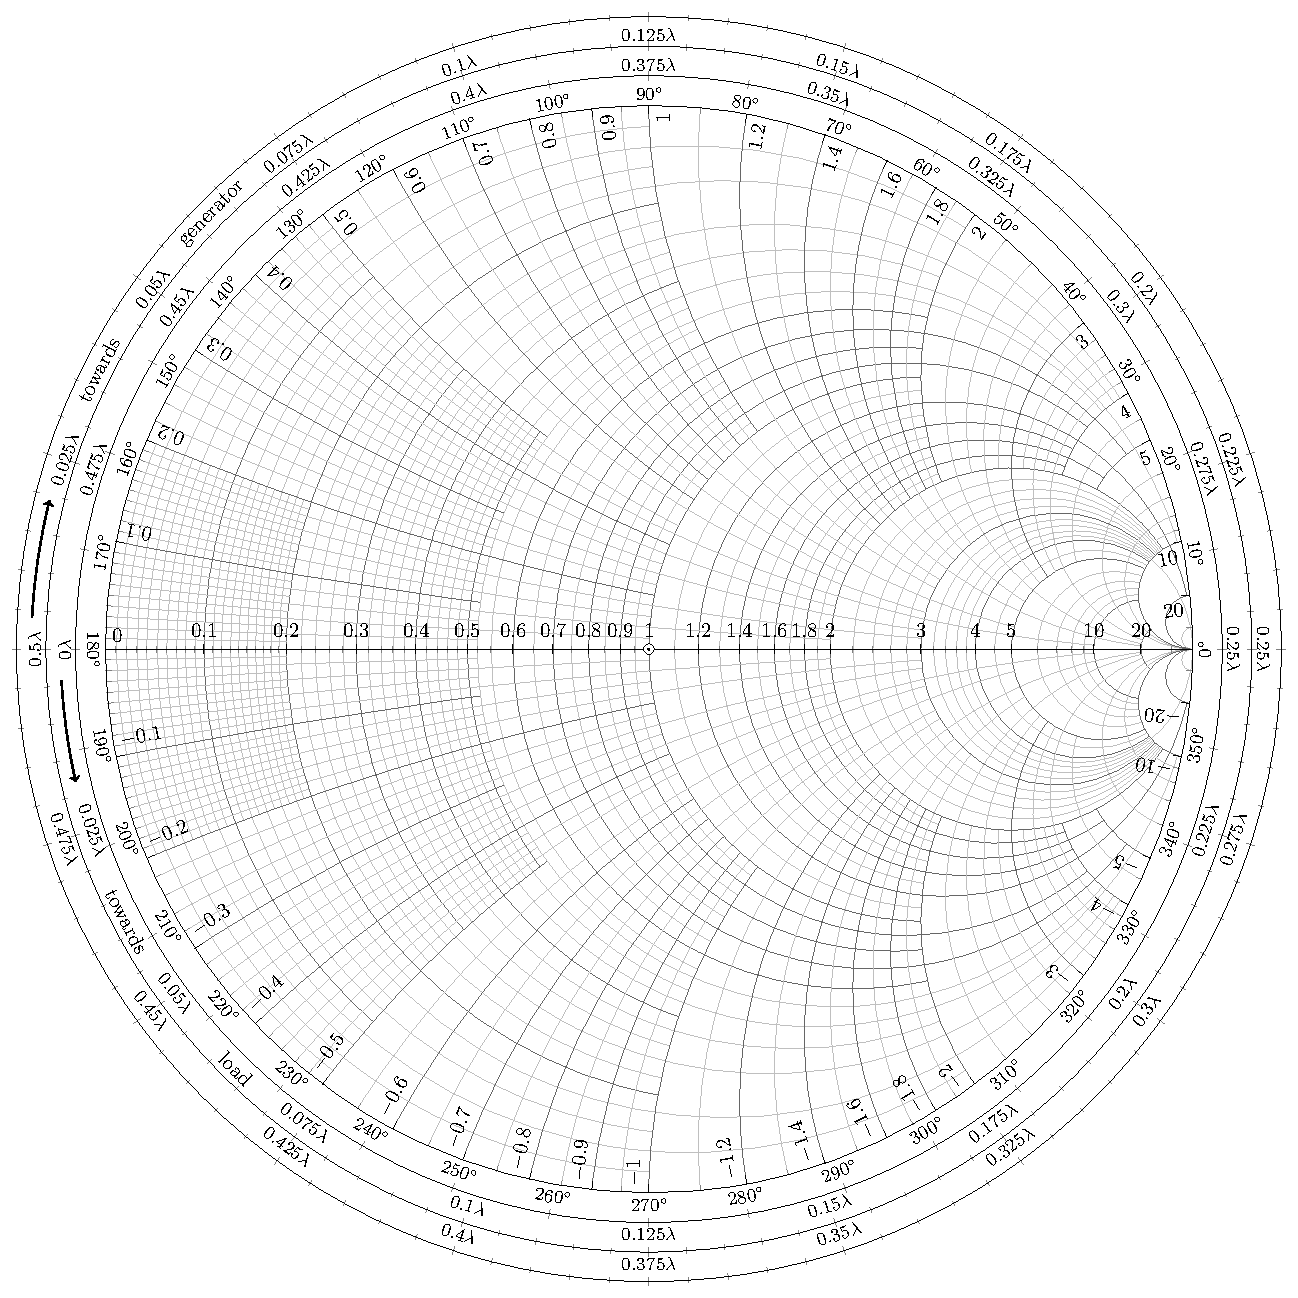
\includegraphics[width=.7\textwidth]{smith.pdf}
% \end{figure}

% \begin{frame}
%   \frametitle{Navigating the Smith Chart}
% \begin{outline}
%   \1 Developed by P Smith in 1939
%   \1 To this day, it is an inte
% \end{outline}
  

% \end{frame}
% \end{frame}
\end{document}
